\comment{
\begin{figure}
(a) DDMS: show state machine, with databases as states and updates as transitions.

(b) DBMS: database sits and waits for queries to arrive; answers them.

(c) Data stream processor: Set of sitting queries; a stream of data passes by.

\caption{Data management systems architectures: DDMS vs. DBMS vs. data stream processors.}
\end{figure}
}

% Should we have an even higher-level overview here, giving a high-level picture of the  DDMS API

DDMSes are update processors.  Data enters the DDMS via its update stream, is processed, incorporated into its persistent state, and the results are passed to the end-user.  Thus the logical abstraction for discussing DDMSes is process-centric: The DDMS represented as a(n infinite) state machine with the machine's state representing an entire relational database at one point in time.

Transitions in this model correspond to modifications of a traditional DBMS' base relations.  This is an important distinction between the DDMS state machine and more traditional interpretations of a state machine; transition functions do not correspond to individual memory operations or CPU instructions, but rather to changes to the inputs of one or more view queries.

Correspondingly, the state of the state machine is organized into a schema of
base relations, materialized views, and other auxiliary datastructures.  We
partition the schema into two components: a \textit{visible schema} containing
materialized representations of the views of interest, and a \textit{auxiliary
schema} containing all of the DDMS' internal machinery (ie, base relations, or
auxiliary materialized views).

Naturally, viewing the database engine as a state machine suggests that we can
precompute each state transition function to make it as efficient as possible. 
Moreover, when ``compiling'' the DDMS, there is no prior state\footnote{This is
not strictly true, we assume that DDMS recompiles are infrequent enough to make
post-compile ``upgrades'' of database state a reasonable requirement} and
latency is not a consideration.  Thus, we are free to use a variety of
compilation tricks unavailable to DBMS optimizers.


\begin{figure}
\begin{center}
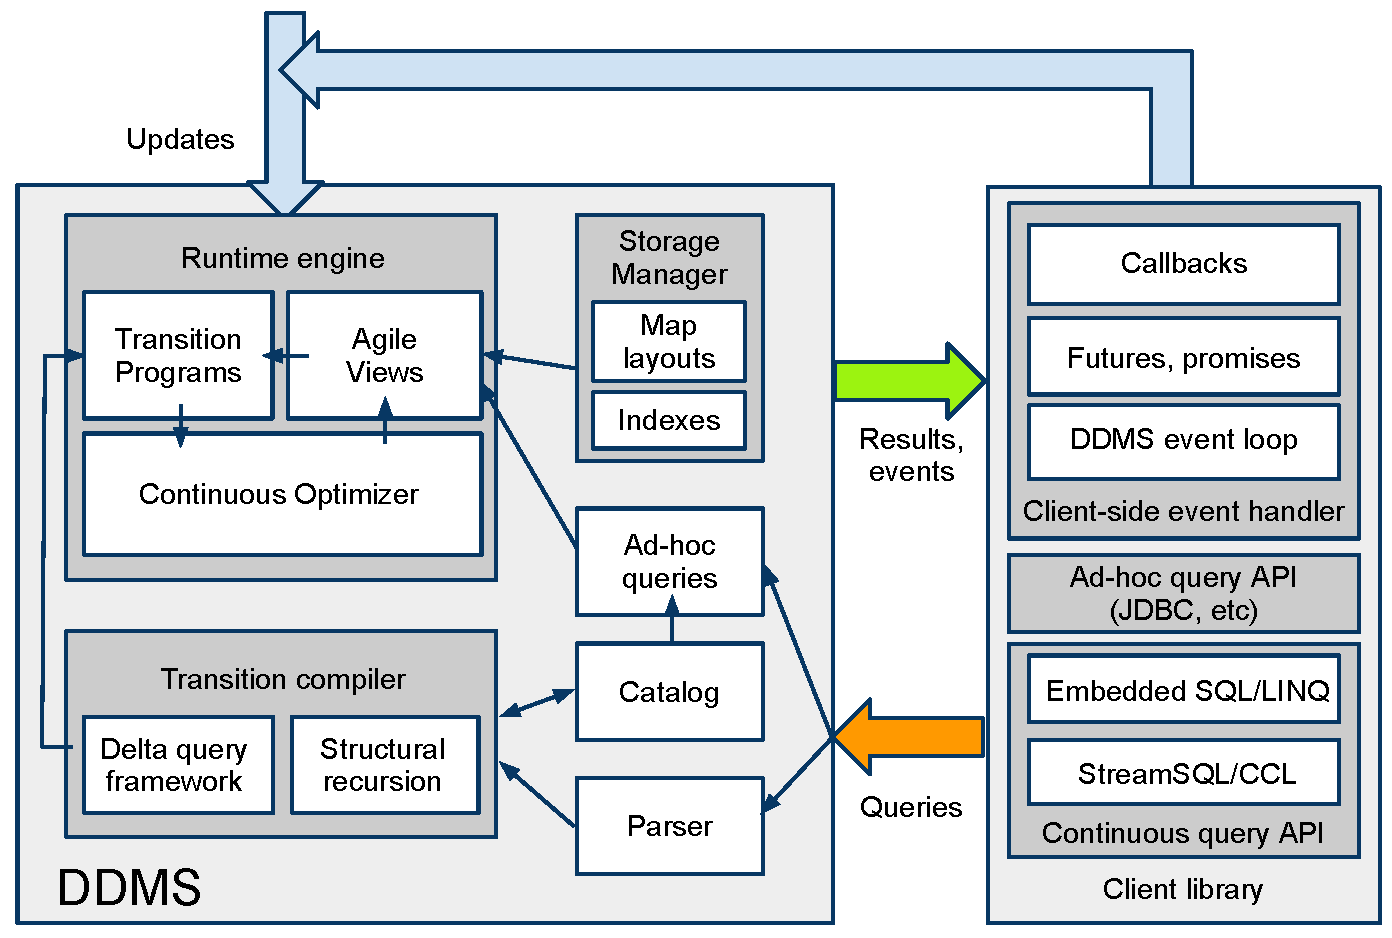
\includegraphics[scale=0.35]{graphics/CIDRarch.pdf}
\end{center}
\caption{Architecture of a Dynamic Data Management System (DDMS)}
\label{fig:ddmsarch}
\end{figure}


\tinysection{DDMS architecture}
Figure~\ref{fig:ddmsarch} provides an architectural design for a DDMS. View
queries and stream queries are specified with embedded SQL or StreamSQL
statements. The application must also specify how the DDMS can invoke
application logic on dynamic results. Unlike JDBC or ODBC interfaces, the key
requirement here is asynchronous result handling, through callbacks, futures and
promises, or via registration on a DDMS event loop and queue. We will also
support ad-hoc queries that can apply standard processing on top of DDMS views,
through an existing DBMS side-by-side with the DDMS handling updates.











Internally, a DDMS is built around the concept of transitioning database state,
and this is realized first and foremost through a transition compiler (discussed
in more detail in the next section). Compilation results in transition programs,
that modify the database state upon update events, comprising the core runtime
engine of a DDMS. The visible and auxiliary views that are part of the state
rely on a storage manager to aid in physical aspects of handling large states,
including implementing a variety of layouts and indexes to facilitate
processing. The runtime includes a continuous query optimizer that guides the
decisions to be made across the database schema, state and storage, in terms of
the cost of applying transitions on updates.










\comment{
Structure of this section:
\begin{itemize}
\item
Mention that viewing the problem in a slightly different way can produce a
dramatically different implementation.


\item
State machine abstraction

\item
Programming model: Boolean views are events, which trigger application code

\item
Architecture diagram:
Compiler/Optimizer: produces low-level view maintenance code.
Update stream.
Event notification facility.
Event notification by invocation by the view maintenance code?
Ad-hoc querying in client-side library?

\item updates can potentially modify many viees

\item
System description.
This really cannot be understood if taken out of context and should be moved to
the following sections.

\begin{itemize}
\item
Query optimization: The next section describes a method of incremental view
maintenance that relies on materializing multiple layers of auxiliary views.
This trades off view maintenance time cost against space cost. The optimizer
will exploit the potential to save space by  deciding which auxiliary view
layers to materialize and which to leave implicit. It will also perform
multi-view optimization, deciding which auxiliary views from different visible
views can be merged.


What do we say about the structural recursion optimization, and where do we say it?

\item
Low-level data structures: we will describe the multi-level hash table data
structure in section 4. Work on parallelization will be required. Our data
structures are a bit unusual since they represent exclusively aggregates and
their values are exclusively numerical. It is a conseqence of our approach that
loops in query processing are always over a set of complete dimensions of the
multi-dimensional table data structures we use; thus all our loops are naturally
implemented as full scans over these dimensions. However, many fields in these
tables will be zero and indexing or compression could be employed to omit
scanning over all-zero areas.

\end{itemize}
\end{itemize}
}


